\section{Accuracy Evaluation}\label{sec:acc_eval}

a mention on differences in measuring accuracy for single-label vs multi
label classifier

mention any metrics that we do not use but are standard, and explain
why we do not use them.

\subsection{Validation Strategy and Sample Space}
mutliple run stratified k-fold cross validation (for enhanced repeatability?).
In effort to reduce sensitivity to chance selection of random samples, all
measurements are performed using stratified 10-fold cross validation.
This gives us a 90/10 train/test split, and is repeated with a new random sample
shuffle 10 times.

For each fold, only the features from the samples selected for training are
used.

A total of 3 batches have been computed and merged, giving 12 species in total.
Selection was performed using the mechanisms outlined in
Section~\ref{sec:sample_select}.
Table~\ref{tbl:used_data} shows the selection of species including spectrogram
and template counts per species.

\begin{table}[!htb]
  \caption{Selected species with spectrogram and template counts}
  \label{tbl:used_data}
  \centering
  \begin{tabular}{l r r}
    Species Label & Spectrograms & Templates \\ \hline
    Common Blackbird           & 20 & 6132\\
    Great Reed Warbler         & 20 & 5111\\
    Common Rosefinch           & 20 & 3191\\
    Common Cuckoo              & 20 & 2909\\
    Common Chiffchaff          & 20 & 2886\\
    European Greenfinch        & 20 & 2759\\
    Pale-breasted Spinetail    & 20 & 2501\\
    Ortolan Bunting            & 20 & 2362\\
    Common Reed Bunting        & 20 & 2233\\
    Chestnut-breasted Wren     & 20 & 2203\\
    Corn Bunting               & 20 & 2082\\
    Rufous-browed Peppershrike & 20 & 1404
  \end{tabular}
\end{table}

\subsection{Accuracy Metrics}
The accuracy is computed for each fold using four standard metrics.
Each accuracy result is stored and then averaged at the end of the 10-fold
cross validation.
The four metrics used are:
\begin{itemize}
  \item \textbf{Accuracy:}
    The ability of the classifier to correctly label samples.
    It is defined as $\frac{TP+TN}{P+N}$;

  \item \textbf{Precision:}
    The ability of the classifier to label 
    It is defined as $\frac{TP}{TP+FP}$;

  \item \textbf{Recall:}
    The ability of the classifier to classify all positive samples correctly.
    It is defined as $\frac{TP}{P}$;

  \item \textbf{F-Beta score:}
    Weighted harmonic mean, or balance, of the precision and recall, where
    higher values indicate better performance.
    It is defined as $\frac{2TP}{2TP+FP+FN}$;
\end{itemize}

Sklearn's |precision_recall_fscore_support| function was used to compute these
metrics.

Because this is a multi-class classification task, each metric must be computed
on a per-label basis, treating the data as a set of binary classification tasks.
To compute scores for the entire classification task, the values must are averaged.
In this case macro averaging is used, in which the mean of each is taken with
equal weighting.
We use macro averaging, in which the mean of the scores are computed with equal
weighting, for each one of the metrics.
Macro averaging is appropriate considering we use stratified k-fold, and each
species is considered equally important to all the others.

\textbf{see about possible multilabel w/o averaging}

Results are promising, good performance has been achieved using the initial
parameters, and improvements are observed after tuning as is shown in
Table~\ref{tbl:acc_before_after}.

\begin{table}
  \centering
  \caption{Comparison of accuracies using default and tuned parameters}
  \label{tbl:acc_before_after}
  \begin{threeparttable}
    \begin{tabular}{l r r}
      & \multicolumn{2}{c}{Metric Scores} \\
      Metric    & Default Params. & Tuned Params. \\ \hline
      Accuracy  & 79.5 (7.3) & 0 \\
      F1 Score  & 77.9 (8.1) & 0 \\
      Recall    & 79.5 (7.4) & 0 \\
      Precision & 82.3 (8.5) & 0
    \end{tabular}
    \begin{tablenotes}
      \footnotesize
      \item[*] Values are shown as percentages.
      \item[*] Standard deviations are shown in parentheses.
    \end{tablenotes}
  \end{threeparttable}
\end{table}

\subsection{AUC curve}
we dont use this but if we can construct one then show how we do and what
this tells us
we probably need to split classification into individual binary classifications.
This should be detailed in the classification section.

\subsection{Confusion Matrix}
A confusion matrix plots the rate at which each label is predicted as any other
label, where the rows represent the true label, and columns represent the
classifier's predictions.

We construct a confusion matrix to evaluate the performance of the classifier
and the features used to discriminate between species.
In this case it is instrumental to show the correlation between bird song of
different species, and shows indications of their similarity of their
vocalisations on the level of granularity defined by the templates extracted.

Figure~\ref{fig:cnf12} shows the resulting confusion matrix from classifying the
selected data, averaged over the 10 folds.

\begin{figure}[!htb]
  \centering
  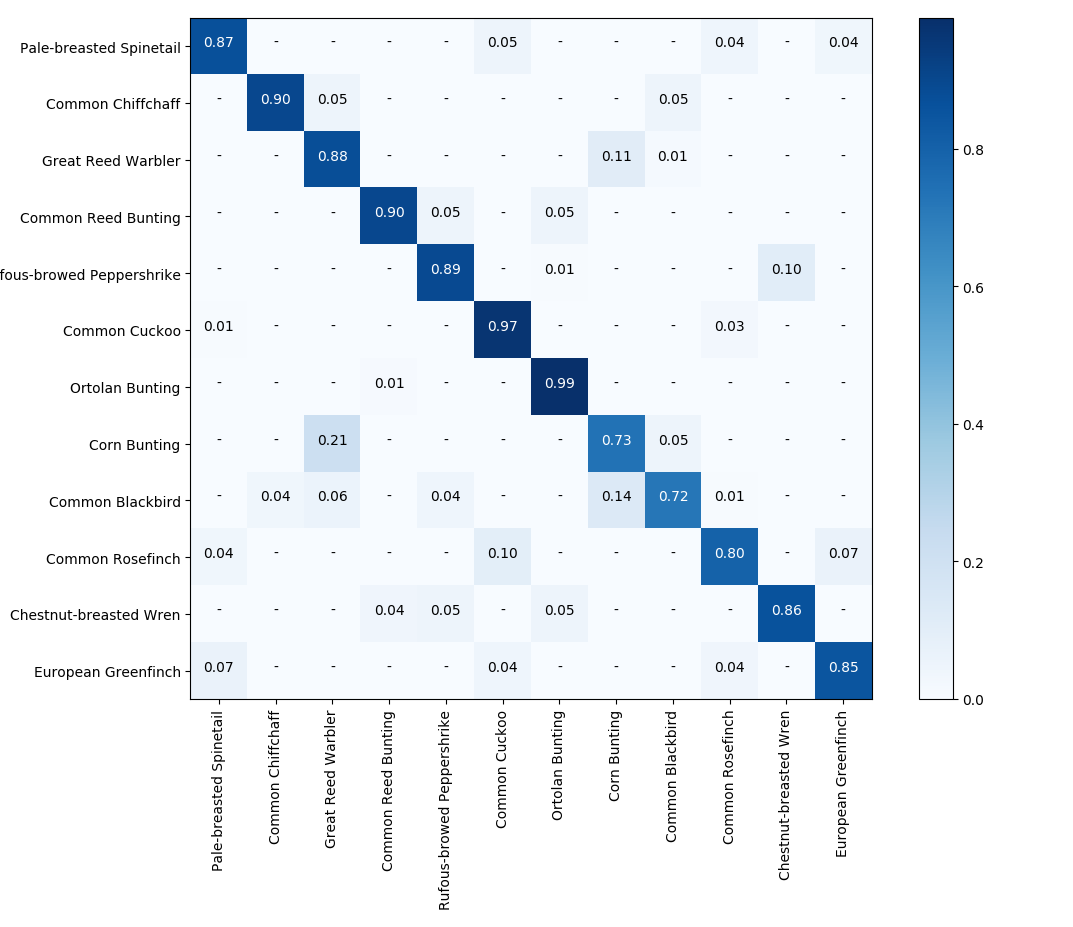
\includegraphics[width=1.0\textwidth]{cnf_matrix_12}
  \caption{Normalized Confusion Matrix}\label{fig:cnf12}
\end{figure}

The confusion matrix shows good classification performance for most species.\\

species A has the highest error-rate, being confused mostly for species B.
This shows that their templates, and therefore their song, share some
similarities.\\

species C has an excellent score, having been confused with no other species.
This shows that species C has very unique vocal characteristics amongst the
picked samples.
